\newpage
\section{Постановка задачи}

\subsection{Цель}
Разработать высокопроизводительный метод рендеринга неявных представлений трёхмерных моделей на основе SDF с использованием возможностей современных графических процессоров.
\subsection{Задачи}
\begin{enumerate}
\item Провести обзор существующих неявных представлений и выбрать базовое представление и базовый метод рендеринга.
\item Разработать алгоритм для визуализации базового представления на основе базового метода рендеринга.
\item Ускорить разработанный алгоритм с использованием аппаратных возможностей современных графических процессоров.
\item Провести его экспериментальную оценку и сравнение с аналогами.
\end{enumerate}

\begin{figure}[ht!] % [ht!] заставляет картинку встать "здесь"
    \centering
    % width=\textwidth растягивает картинку на всю ширину текста
    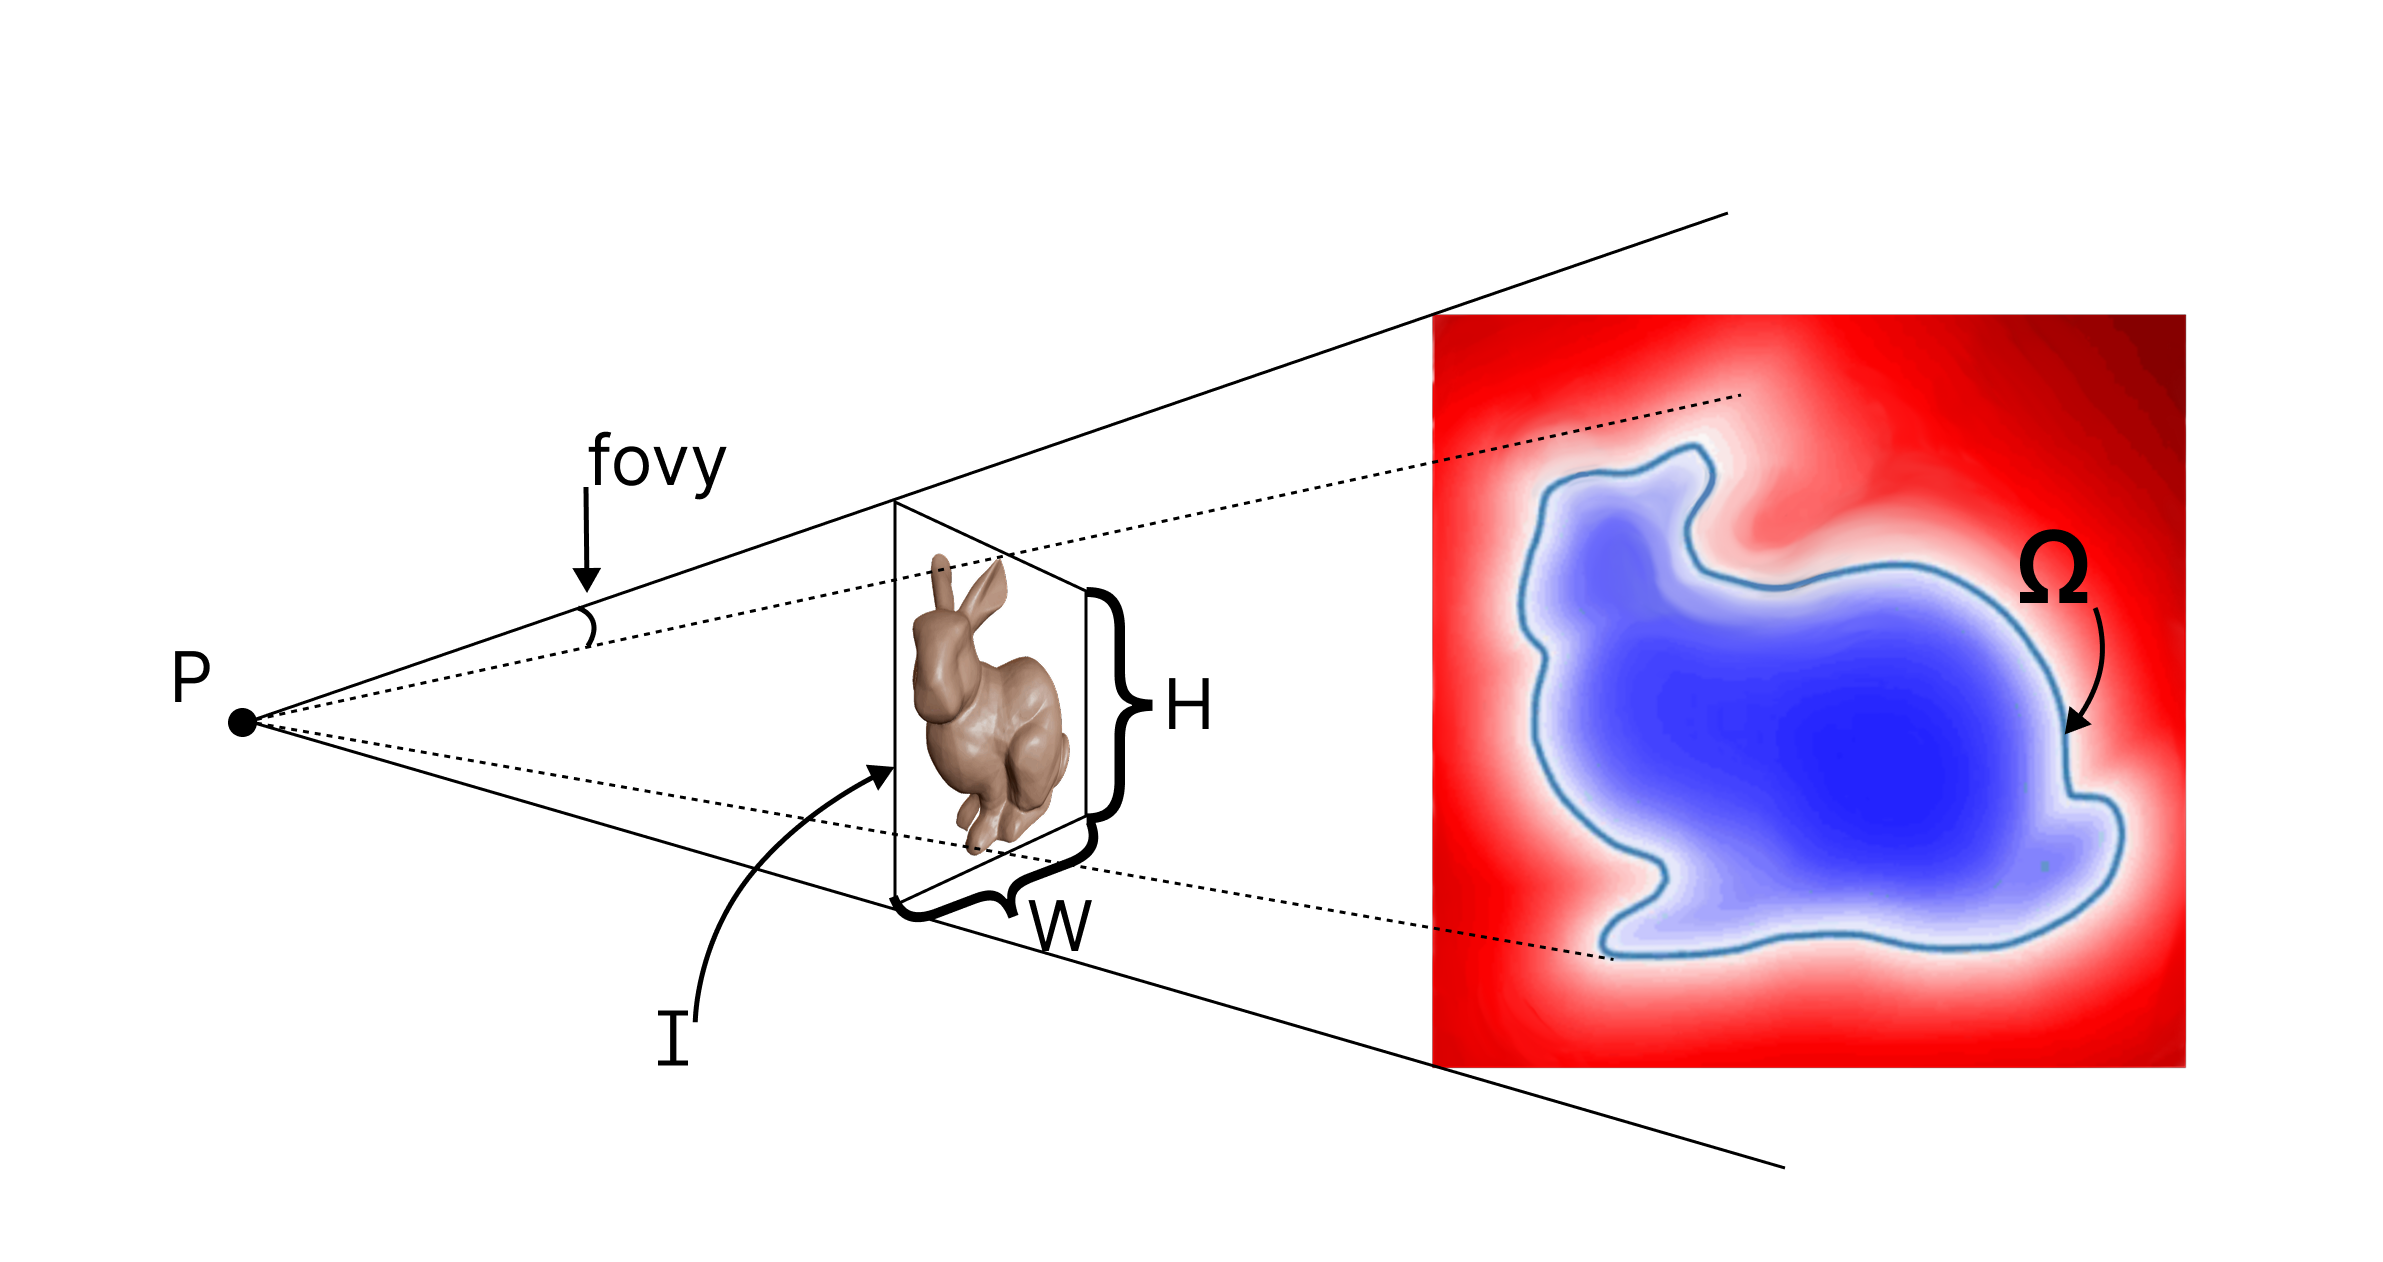
\includegraphics[width=0.6\textwidth]{figures/formal.png} 
    \caption{Иллюстрация к формальной постановке задачи}
    \label{fig:fullwidth}
\end{figure}

\newpage

\subsection{Формальная постановка задачи}

\paragraph{Вход.}
Задана ограниченная поверхность \(\Omega \subset \mathbb{R}^3\),
представленная как нулевая изоповерхность функции знакового расстояния
\[
\Omega = \{\, x \in \mathbb{R}^3 \mid \operatorname{SDF}(x) = 0 \,\}.
\]

Для любой точки \(x \in \mathbb{R}^3\) расстояние до границы \(\partial\Omega\) задаётся как
\[
d(x,\partial\Omega) = \inf_{y \in \partial\Omega} \lVert x - y \rVert_2 \in \mathbb{R}_{\ge 0}.
\]
Тогда функция знакового расстояния определяется выражением
\[
\operatorname{SDF}(x) =
\begin{cases}
 d(x,\partial\Omega),   & x \notin \Omega,\\[2pt]
 0,                     & x \in \partial\Omega,\\[2pt]
 -d(x,\partial\Omega),  & x \in \Omega.
\end{cases}
\]

Определена камера $C$, задающая условия наблюдения сцены:
\[
C = \langle P, \vec{d}, fovy, a \rangle,
\]
где:
\begin{itemize}
    \item $P \in \mathbb{R}^3$ — положение оптического центра камеры;
    \item $\vec{d} = (\theta, \phi)$ — направление главной оптической оси, заданное сферическими углами;
    \item $fovy \in (0, \pi)$ — вертикальный угол поля зрения;
\end{itemize}

\paragraph{Выход.}
Требуется получить RGB-изображение для камеры $C$:
\[
I \in \mathbb{R}^{W \times H \times 3},
\]
где \(W,H \in \mathbb{N}\) --- его ширина и высота.

